\documentclass[compress]{beamer}        % [compress] (written before {beamer} <=> navigation bar one line, all subsections in 1 line instead of 2

% Setup appearance:
\usetheme{CambridgeUS}
%	AnnArbor | Antibes | Bergen |
%	Berkeley | Berlin | Boadilla |
%	boxes | CambridgeUS | Copenhagen |
%	Darmstadt | default | Dresden |
%	Frankfurt | Goettingen |Hannover |
%	Ilmenau | JuanLesPins | Luebeck |
%	Madrid | Malmoe | Marburg |
%	Montpellier | PaloAlto | Pittsburgh |
%	Rochester | Singapore | Szeged |
%	Warsaw
%

\useoutertheme[footline=authorinstitute,subsection=false]{miniframes}
\usecolortheme{whale}

%	albatross | beaver | beetle |
%	crane | default | dolphin |
%	dove | fly | lily | orchid |
%	rose |seagull | seahorse |
%	sidebartab | structure |
%	whale | wolverine


\setbeamertemplate{footline}
{
  \hbox{%
  \begin{beamercolorbox}[wd=.25\paperwidth,ht=2.25ex,dp=1ex,center]{title in head/foot}%
    \usebeamerfont{date in head/foot}\insertshortauthor
  \end{beamercolorbox}%
  \begin{beamercolorbox}[wd=.5\paperwidth,ht=2.25ex,dp=1ex,center]{date in head/foot}%
    \usebeamerfont{title in head/foot}\insertshortinstitute
  \end{beamercolorbox}%
  \begin{beamercolorbox}[wd=.25\paperwidth,ht=2.25ex,dp=1ex,center]{title in head/foot}%
    \usebeamerfont{date in head/foot}
    \insertframenumber{} / \inserttotalframenumber
  \end{beamercolorbox}}%
  \vskip0pt%
}

%\setbeamercolor{titlelike}{parent=structure}
%\setbeamercolor{structure}{fg=beamer@blendedblue}
%% \useinnertheme{rounded}
%\setbeamerfont{block title}{size={}}
%\usefonttheme[onlylarge]{structurebold}   % title and words in the table of contents bold
%\setbeamerfont*{frametitle}{size=\normalsize,series=\bfseries}
\setbeamertemplate{navigation symbols}{}
\setbeamercolor{frametitle}{parent=boxes, bg=white}


% Standard packages

\usepackage[english]{babel}
\usepackage[latin1]{inputenc}
\usepackage{times}
\usepackage[T1]{fontenc}
\usepackage{amsbsy}         % for \boldsymbol command (bold in math mode)
\usepackage{amsfonts, amssymb}
\usepackage{epsfig}
\usepackage{color}
\definecolor{camblue}{RGB}{26,26,89}
\definecolor{Rblue}{RGB}{0,255,255}
\definecolor{Rdarkblue}{RGB}{0,0,255}
\definecolor{Rgreen}{RGB}{0,205,0}
\newcommand{\tcb}{\textcolor{beamer@blendedblue}}
\newcommand{\tcbb}{\textcolor{camblue}}
\newcommand{\tcr}{\textcolor{red}}
\newcommand{\tcg}{\textcolor{gray}}
\newcommand{\tcRg}{\textcolor{Rgreen}}
\newcommand{\tcRdb}{\textcolor{Rdarkblue}}
\newcommand{\tcRb}{\textcolor{Rblue}}
\newcommand{\sq}{\begin{eqnarray}}
\newcommand{\fq}{\end{eqnarray}}
\newcommand{\bp}{$\bullet$\:}


%%%%%%%%%%%%%%%%%%%%%%%%%%%%%%%%%%%%%%%%%%%%%%%%%%%%%%%%%%%%%%%%%%%%%%%%%%%%%%%%%%%%%%%%%%%%%
% THIS IS WHERE THE DOCUMENT BEGINS


%\setbeamercovered{transparent}   % overlays with light grey 1st slide
\title
{
{\huge Title\\[0.3cm] }
}
\author[Kevin O'Brien]{{\bf Author}}
\institute[University of Limerick, Maths \& Stats Dept]{}
\date{}

\begin{document}

\begin{frame}
\huge
\[ \mbox{Method Comparison Studies with \texttt{R}} \]
\Large
\[ \mbox{Kevin O'Brien} \]
\end{frame}
\begin{frame}
\setcounter{tocdepth}{1}
\tableofcontents
\end{frame}

\section{Additional Remarks on Bland-Altman Analysis (Optional)}
\begin{frame}
\textbf{Section 3: Additional Remarks on Bland-Altman Analysis}
\begin{itemize}
\item Popularity of the Bland-Altman Method
\item Treatment of Outliers
\item Regression Based Calculation of LoA
\item Bartko's Ellipse
\item Coefficient of Repeatability
\end{itemize}
\end{frame}
\subsection{Popularity of the Bland-Altman Method}
%------------------------------------------------------------------------%

\begin{frame}{\bf \tcb{The Bland-Altman Plot: Prevalence}}
\begin{itemize}\itemsep0.7cm

\item Limits of Agreement are used extensively in medical literature for assessing agreement between two methods.
\item According to Google Scholar, Bland and Altman's 1986 paper has 22,456 citations. \\(``The Pricing of Options and Corporate Liabilities" by Black and Scholes has 19,019 citations.)
\end{itemize}
\end{frame}

\begin{frame}
\frametitle{Popularity of the Bland-Altman Method}


\begin{itemize}
\item This methodology, now commonly known as
the `Bland-Altman Plot', has proved very successful.
\alert{BA86}, which further develops the methodology, was found
to be the sixth most cited paper of all time by the
\alert{BAcite}.
\item \alert{Dewitte} also commented on the rate at which
prevalence of the Bland-Altman plot has developed in scientific
literature. 
\item The Bland-Altman Plot has since become expected, and
often obligatory, approach for presenting method comparison
studies in many scientific journals \alert{hollis}. Furthermore
\item \alert{BritHypSoc} recommend its use in papers pertaining to
method comparison studies for the journal of the British
Hypertension Society.
\end{itemize}
\end{frame}

\subsection{Regression Techniques}
%%%%%%%%%%%%%%%%%%%%%%%%%%%%%%%%%%%%%%%%%%%%%%%%%%%%%%%%%%%%%%%%%%%%%%%%%%%%%%%%%%%%%%
\begin{frame}
\begin{itemize}
\item Application of regression techniques to the Bland-Altman plot, and
subsequent formal testing for the constant variability of
differences is informative.
\item  The data set may be divided into two
subsets, containing the observations wherein the difference values
are less than and greater than the inter-method bias respectively.
\item For both of these fits, hypothesis tests for the respective slopes
can be performed. While both tests can be considered separately,
multiple comparison procedures, such as the Benjamini-Hochberg
\alert{BH} test, should be also be used.
\end{itemize}
\end{frame}

\subsection{Treatment of Outliers}
%%%%%%%%%%%%%%%%%%%%%%%%%%%%%%%%%%%%%%%%%%%%%%%%%%%%%%%%%%%%%%%%%%%%%%%%%%%%%%%%%%%%%%
\begin{frame}
\frametitle{Outliers with Bland-Altman Plots}
\begin{itemize}
\item The Bland-Altman plot also can be used to identify outliers. An
outlier is an observation that is conspicuously different from the
rest of the data that it arouses suspicion that it occurs due to a
mechanism, or 

conditions, different to that of the rest of the
observations. 
\item Classification of outliers can be determined with
numerous established approaches, such as the Grubb's test, but
always classification must be informed by the logic of the data's
formulation. Figure 1.6 is a Bland-Altman plot with two potential
outliers.
\end{itemize}




\end{frame}
%%%%%%%%%%%%%%%%%%%%%%%%%%%%%%%%%%%%%%%%%%%%%%%%%%%%%%%%%%%%%%%%%%%%%%%%%%%%%%%%%%%%%%
\begin{frame}
\frametitle{Outliers with Bland-Altman Plots}
\alert{BA99} do not recommend excluding outliers from analyses,
but remark that recalculation of the inter-method bias estimate,
and further calculations based upon that estimate, are useful for
assessing the influence of outliers. The authors remark that `we
usually find that this method of analysis is not too sensitive to
one or two large outlying differences'.

\end{frame}
%%%%%%%%%%%%%%%%%%%%%%%%%%%%%%%%%%%%%%%%%%%%%%%%%%%%%%%%%%%%%%%%%%%%%%%%%%%%%%%%%%%%%%
\begin{frame}
\frametitle{Outliers with Bland-Altman Plots}
%\alert{Grubbs} defined an outlier as a co-variate that appears to
%deviate markedly from other members of the sample in which it
%occurs.

In classifying whether a observation from a univariate data set is
an outlier, Grubbs' outlier test is widely used. In assessing
whether a co-variate in a Bland-Altman plot is an outlier, this
test is useful when applied to the difference values treated as a
univariate data set. For Grubbs' data, this outlier test is
carried out on the differences, yielding the following results.
\end{frame}
%%%%%%%%%%%%%%%%%%%%%%%%%%%%%%%%%%%%%%%%%%%%%%%%%%%%%%%%%%%%%%%%%%%%%%%%%%%%%%%%%%%%%%
\begin{frame}
\frametitle{Outliers with Bland-Altman Plots}
The null and alternative hypotheses is the absence and presence of
at least one outlier respectively. Grubbs' outlier test statistic
$G$ is the largest absolute deviation from the sample mean divided
by the standard deviation of the differences. For the `F vs C'
comparison, $G = 3.6403$. The critical value is calculated using
Student's $t$ distribution and the sample size,
\begin{equation}
U = \frac{n-1}{\sqrt{n}} \sqrt{\frac{t_{\alpha/(2n),n-2}^2}{n - 2
+ t_{\alpha/(2n),n-2}^2}}.
\end{equation}
\end{frame}

%%%%%%%%%%%%%%%%%%%%%%%%%%%%%%%%%%%%%%%%%%%%%%%%%%%%%%%%%%%%%%%%%%%%%%%%%%%%%%%%%%%%%%
\begin{frame}
\frametitle{Outliers with Bland-Altman Plots}
For this test $U = 0.7501$. The conclusion of this test is that
the fourth observation in the `F vs C' comparison is an outlier,
with $p-value = 0.002799$.
\end{frame}
%%%%%%%%%%%%%%%%%%%%%%%%%%%%%%%%%%%%%%%%%%%%%%%%%%%%%%%%%%%%%%%%%%%%%%%%%%%%%%%%%%%%%%
\frametitle{Bartko's Ellipse}
\begin{frame}
As a complement to the Bland-Altman plot, \alert{Bartko} proposes
the use of a bivariate confidence ellipse, constructed for a
predetermined level.

The minor axis relates to the between subject variability, whereas
the major axis relates to the error mean square, with the ellipse
depicting the size of both relative to each
other.
\end{frame}
%%%%%%%%%%%%%%%%%%%%%%%%%%%%%%%%%%%%%%%%%%%%%%%%%%%%%%%%%%%%%%%%%%%%%%%%%%%%%%%%%%%%%%
\begin{frame}

\alert{AltmanEllipse} provides the relevant calculations for
the ellipse. Bartko states that the ellipse can, inter alia, be
used to detect the presence of outliers (furthermore
\alert{Bartko} proposes formal testing procedures, that shall be
discussed in due course). Inspection of Figure 1.7 shows that the
fourth observation is outside the bounds of the ellipse,
concurring with the conclusion that it is an outlier.
\end{frame}

%%%%%%%%%%%%%%%%%%%%%%%%%%%%%%%%%%%%%%%%%%%%%%%%%%%%%%%%%%%%%%%%%%%%%%%%%%%%%%%%%%%%%%
\begin{frame}

\begin{figure}[h!]
  % Requires \usepackage{graphicx}
  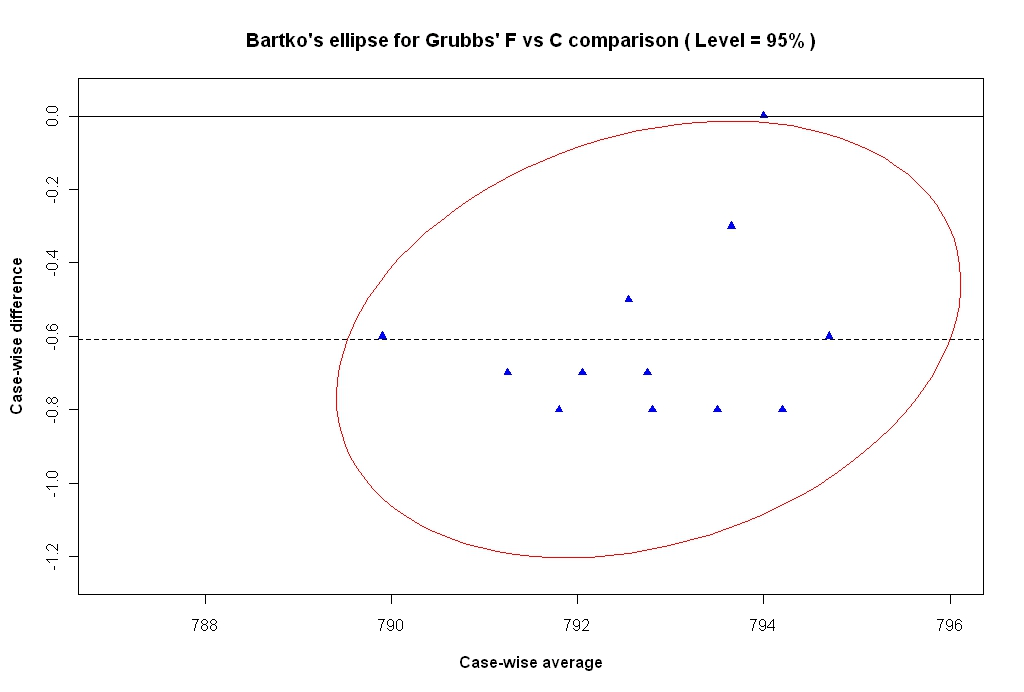
\includegraphics[width=130mm]{GrubbsBartko.jpeg}
  \caption{Bartko's Ellipse For Grubbs' Data.}\label{GrubbsBartko}
\end{figure}
\end{frame}
%%%%%%%%%%%%%%%%%%%%%%%%%%%%%%%%%%%%%%%%%%%%%%%%%%%%%%%%%%%%%%%%%%%%%%%%%%%%%%%%%%%%%%
\begin{frame}
The limitations of using bivariate approaches to outlier detection
in the Bland-Altman plot can demonstrated using Bartko's ellipse.
A co-variate is added to the `F vs C' comparison that has a
difference value equal to the inter-method bias, and an average
value that markedly deviates from the rest of the average values
in the comparison, i.e. 786. 
\end{frame}

%%%%%%%%%%%%%%%%%%%%%%%%%%%%%%%%%%%%%%%%%%%%%%%%%%%%%%%%%%%%%%%%%%%%%%%%%%%%%%%%%%%%%%
\begin{frame}
Table 1.8 depicts a $95\%$ confidence
ellipse for this enhanced data set. By inspection of the
confidence interval, a conclusion would be reached that this extra
co-variate is an outlier, in spite of the fact that this
observation is consistent with the intended conclusion of the
Bland-Altman plot.
\end{frame}

%%%%%%%%%%%%%%%%%%%%%%%%%%%%%%%%%%%%%%%%%%%%%%%%%%%%%%%%%%%%%%%%%%%%%%%%%%%%%%%%%%%%%%
\begin{frame}
\begin{figure}[h!]
  % Requires \usepackage{graphicx}
  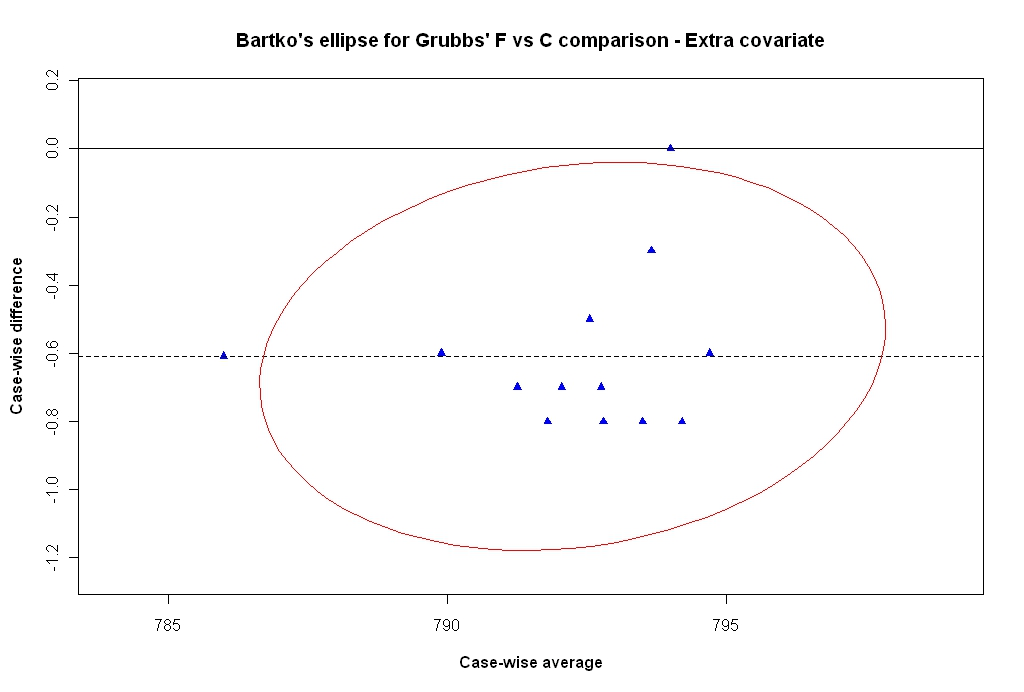
\includegraphics[width=130mm]{GrubbsBartko2.jpeg}
  \caption{Bartko's Ellipse For Grubbs' Data, with an extra covariate.}\label{GrubbsBartko2}
\end{figure}
\end{frame}

%%%%%%%%%%%%%%%%%%%%%%%%%%%%%%%%%%%%%%%%%%%%%%%%%%%%%%%%%%%%%%%%%%%%%%%%%%%%%%%%%%%%%%
\begin{frame}
In the Bland-Altman plot, the horizontal displacement of any
observation is supported by two independent measurements. Any
observation should not be considered an outlier on the basis of a
noticeable horizontal displacement from the main cluster, as in
the case with the extra co-variate. Conversely, the fourth
observation, from the original data set, should be considered an
outlier, as it has a noticeable vertical displacement from the
rest of the observations.
\end{frame}

%%%%%%%%%%%%%%%%%%%%%%%%%%%%%%%%%%%%%%%%%%%%%%%%%%%%%%%%%%%%%%%%%%%%%%%%%%%%%%%%%%%%%%
\begin{frame}
Bartko's ellipse provides a visual aid to determining the
relationship between variances. If $\mbox{var}(a_{i})$ is greater
than $\mbox{var}(d_{i})$, the orientation of the ellipse is
horizontal. Conversely if $\mbox{var}(a_{i})$ is less than
$\mbox{var}(d_{i})$, the orientation of the ellipse is vertical.
\end{frame}


%\begin{figure}[h!]
%\begin{center}
%  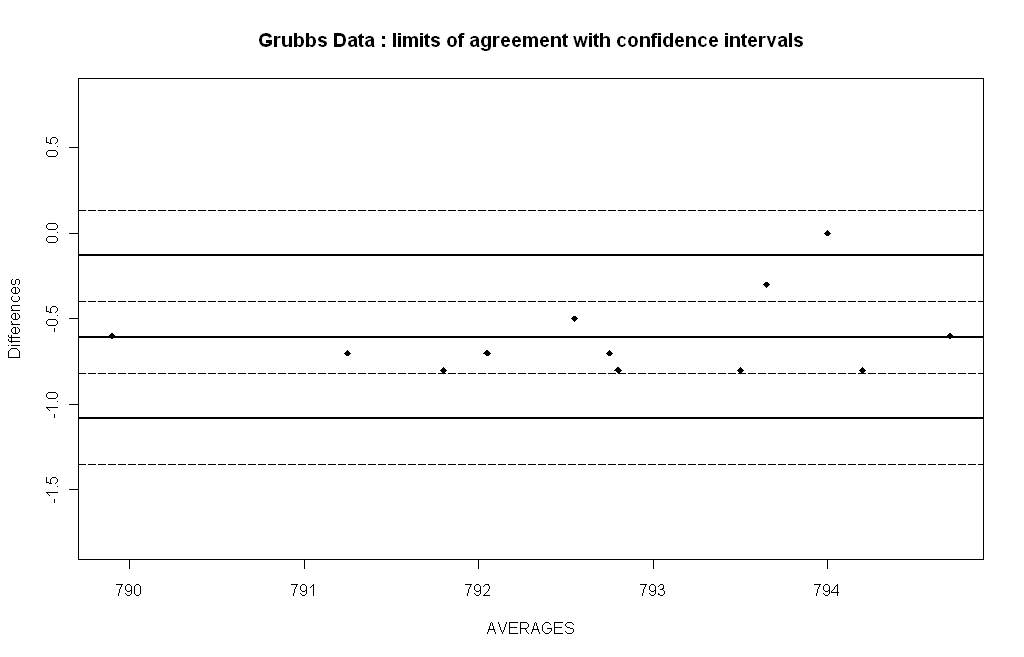
\includegraphics[width=125mm]{GrubbsLOAwCIs.jpeg}
%  \caption{Limits of agreement with confidence intervals}\label{LOAwCIs}
%\end{center}
%\end{figure}

%%%%%%%%%%%%%%%%%%%%%%%%%%%%%%%%%%%%%%%%%%%%%%%%%%%%%%%%%%%%%%%%%%%%%%%%%%%%%%%%%%%%%%

\subsection{Variations of the Bland-Altman Plot (optional)}
\begin{frame}
Referring to the
assumption that bias and variability are constant across the range
of measurements, \alert{BA99} address the case where there is an
increase in variability as the magnitude increases. They remark
that it is possible to ignore the issue altogether, but the limits
of agreement would wider apart than necessary when just lower
magnitude measurements are considered. 
\end{frame}

%%%%%%%%%%%%%%%%%%%%%%%%%%%%%%%%%%%%%%%%%%%%%%%%%%%%%%%%%%%%%%%%%%%%%%%%%%%%%%%%%%%%%%
\begin{frame}
Conversely the limits would
be too narrow should only higher magnitude measurements be used.
To address the issue, they propose the logarithmic transformation
of the data. The plot is then formulated as the difference of
paired log values against their mean. Bland and Altman acknowledge
that this is not easy to interpret, and may not be suitable in
all cases.
\end{frame}
%%%%%%%%%%%%%%%%%%%%%%%%%%%%%%%%%%%%%%%%%%%%%%%%%%%%%%%%%%%%%%%%%%%%%%%%%%%%%%%%%%%%%%
\begin{frame}

\alert{BA99} offers two variations of the Bland-Altman plot that
are intended to overcome potential problems that the conventional
plot would inappropriate for. The first variation is a plot of
casewise differences as percentage of averages, and is appropriate
when there is an increase in variability of the differences as the
magnitude increases. 
\end{frame}
%%%%%%%%%%%%%%%%%%%%%%%%%%%%%%%%%%%%%%%%%%%%%%%%%%%%%%%%%%%%%%%%%%%%%%%%%%%%%%%%%%%%%%
\begin{frame}
The second variation is a plot of casewise
ratios as percentage of averages. This will remove the need for
log transformation. This approach is useful when there is an
increase in variability of the differences as the magnitude of the
measurement increases. \alert{Eksborg} proposed such a ratio plot,
independently of Bland and Altman. \alert{Dewitte} commented on
the reception of this article by saying `Strange to say,this
report has been overlooked'.

\end{frame}

%%%%%%%%%%%%%%%%%%%%%%%%%%%%%%%%%%%%%%%%%%%%%%%%%%%%%%%%%%%%%%%%%%%%%%%%%%%%%%%%%%%%%%
\begin{frame}

\subsection*{Regression-based Limits of Agreement (optional)} Assuming that
there will be no curvature in the scatter-plot, the methodology
regresses the difference of methods ($d$) on the average of those
methods ($a$) with a simple intercept slope model; $\hat{d} =
b_{0}+ b_{1}a.$ Should the slope $b_{1}$ be found to be
negligible, $\hat{d}$ takes the value $\bar{d}$.

The next step to take in calculating the limits is also a
regression, this time of the residuals as a function of the scale
of the measurements, expressed by the averages $a_{i}$;
 $ \hat{R} = c_{0}+ c_{1}a_{i}$
\end{frame}

%%%%%%%%%%%%%%%%%%%%%%%%%%%%%%%%%%%%%%%%%%%%%%%%%%%%%%%%%%%%%%%%%%%%%%%%%%%%%%%%%%%%%%
\begin{frame}
With reference to absolute values following a half-normal
distribution with mean $\sigma\sqrt{\frac{2}{\pi}}$, \alert{BA99} formulate the regression based limits of agreement as
follows
 \begin{equation}
  \hat{d} \pm 1.96\sqrt{\frac{\pi}{2}}\hat{R} = \hat{d} \pm 2.46\hat{R}
 \end{equation}

\end{frame}

%%%%%%%%%%%%%%%%%%%%%%%%%%%%%%%%%%%%%%%%%%%%%%%%%%%%%%%%%%%%%%%%%%%%%%%%%%%%%%%%%%%%%%
\section{Formal Methods (Optional)}

\begin{frame}
\frametitle{Formal Methods}

\textbf{Section 3 - Formal Methods}
\begin{itemize}
\item
\item
\end{itemize}

\end{frame}

\begin{frame}
\frametitle{Formal Methods}
\begin{itemize}
\item The approach proposed by \alert{BA83} is a formal test on the
Pearson correlation coefficient of case-wise differences and means
($\rho_{ad}$).
\item According to the authors, this test is equivalent
to the `Pitman Morgan Test'. For the Grubbs data, the correlation
coefficient estimate ($r_{ad}$) is 0.2625, with a 95\% confidence
interval of (-0.366, 0.726) estimated by Fishers `r to z'
transformation \alert{Cohen}.
\end{itemize}
 
\end{frame}
%%%%%%%%%%%%%%%%%%%%%%%%%%%%%%%%%%%%%%%%%%%%%%%%%%%%%%%%%%%%%%%%%%%%%%%%%%%%%%%%%%%%%%
\begin{frame}
\frametitle{Formal Methods}
\begin{itemize}
\item The null hypothesis ($\rho_{ad}$
=0)would fail to be rejected. Consequently the null hypothesis of
equal variances of each method would also fail to be rejected.
There has no been no further mention of this particular test in
\alert{BA86}, although \alert{BA99} refers to Spearman's rank
correlation coefficient. 
\item \alert{BA99} comments `we do not see a
place for methods of analysis based on hypothesis testing'.
\alert{BA99} also states that consider structural equation models
to be inappropriate.
\end{itemize}
 
\end{frame}
%%%%%%%%%%%%%%%%%%%%%%%%%%%%%%%%%%%%%%%%%%%%%%%%%%%%%%%%%%%%%%%%%%%%%%%%%%%%%%%%%%%%%%
\begin{frame}
\frametitle{Formal Methods}
\alert{DunnSEME} highlights an important issue regarding using
models such as these, the identifiability problem. This comes as a
result of there being too many parameters to be estimated.
Therefore assumptions about some parameters, or estimators used,
must be made so that others can be estimated. For example $\alpha$
may take the value of the inter-method bias estimate from
Bland-Altman methodology. Another assumption is that the precision
ratio $\lambda=\frac{\sigma^{2}_{\epsilon}}{\sigma^{2}_{\delta}}$
may be known.
\end{frame}
%%%%%%%%%%%%%%%%%%%%%%%%%%%%%%%%%%%%%%%%%%%%%%%%%%%%%%%%%%%%%%%%%%%%%%%%%%%%%%%%%%%%%%
\begin{frame}
\frametitle{Formal Methods}
\alert{DunnSEME} considers methodologies based on two methods with single measurements on each subject as inadequate for a serious study
on the measurement characteristics of the methods. This is because there would not be enough data to allow for a meaningful analysis.
There is, however, a contrary argument that is very difficult to get replicate
observations when the measurement method requires invasive medical procedure.
\end{frame}
%%%%%%%%%%%%%%%%%%%%%%%%%%%%%%%%%%%%%%%%%%%%%%%%%%%%%%%%%%%%%%%%%%%%%%%%%%%%%%%%%%%%%%
\begin{frame}
\frametitle{Formal Methods}
\alert{DunnSEME} recommends the following approach for analyzing
method comparison data. Firstly he recommends conventional
Bland-Altman methodology; plotting the scatterplot and the
Bland-Altman plot, complemented by estimate for the limits of
agreement and the correlation coefficient between the difference
and the mean. Additionally boxplots may be useful in considering
the marginal distributions of the observations. The second step is
the calculations of summary statistics; the means and variances of
each set of measurements, and the covariances.
%Should covariance values be greater than the either of the two variances,
\end{frame}
%%%%%%%%%%%%%%%%%%%%%%%%%%%%%%%%%%%%%%%%%%%%%%%%%%%%%%%%%%%%%%%%%%%%%%%%%%%%%%%%%%%%%%
\begin{frame}
\frametitle{Formal Methods}
When both methods measure in the same scale (i.e. $\beta = 1$),
\alert{DunnSEME} recommends the use of Grubbs estimators to
estimate error variances, and to test for their equality. A test
of whether the intercept $\alpha$ may be also be appropriate.



%This application of the
%Grubbs method presumes the existence of this condition, and necessitates
%replication of observations by means external to and independent of the first
%means. The Grubbs estimators method is based on the laws of propagation of
%error. By making three independent simultaneous measurements on the same
%physical material, it is possible by appropriate mathematical manipulation of
%the sums and differences of the associated variances to obtain a valid
%estimate of the precision of the primary means. Application of the Grubbs
%estimators procedure to estimation of the precision of an apparatus uses
%the results of a physical test conducted in such a way as to obtain a series
%of sets of three independent observations.


\end{frame}
\section{Hamlett}
%--------------------------------------------------------------------------------------------------------%
%Include a Short Section on Hamlett in the notes - for reading after the talk

\begin{frame}
\frametitle{Hmalett}
\large

\begin{itemize}
\item Hamlett re-analyses the data of \textbf{Lam} to generalize their model to cover other settings not covered by the Lam method.

\item In many cases, repeated observation are collected from each subject in sequence  and/or longitudinally.


\[ y_i = \alpha + \mu_i + \epsilon \]
\end{itemize}

\end{frame}
%--------------------------------------------------------------------------------------------------------%


\begin{frame}
\frametitle{Hmalett}
The classical model is based on measurements $y_{mi}$
by method $m=1,2$ on item $i = 1,2 \ldots$

\[y_{mi} + \alpha_{m} + \mu_{i} + e_{mi}\]

\[e_{mi} \sim \mathcal{n} (0,\sigma^2_m)\]

Even though the separate variances can not be
identified, their sum can be estimated by the empirical variance of the differences.

Like wise the separate $\alpha$ can not be
estimated, only theiir difference can be estimated as
$\bar{D}$

\end{frame}
%%%%%%%%%%%%%%%%%%%%%%%%%%%%%%%%%%%%%%%%%%%%%%%%%%%%%%%%%%%%%%%%%%%%%%%%%%%%%%%%%%%%%%

%%%%%%%%%%%%%%%%%%%%%%%%%%%%%%%%%%%%%%%%%%%%%%%%%%%%%%%%%%%%%%%%%%%%%%%%%%%%%%%%%%%%%%%%%%%%%%%%%%%%%%%%
%-----------------------------------------------------------------------------------%
\begin{frame}
\frametitle{Remarks on the Multivariate Normal Distribution}
\begin{itemize}
\item Diligence is required when considering the models. Carstensen specifies his models in terms of the univariate normal distribution. \item Roy's model is specified using the bivariate normal distribution.
\item 
This gives rises to a key difference between the two model, in that a bivariate model accounts for covariance between the variables of interest.
\end{itemize}
\end{frame}
%----------------------------------------------------------%
%-----------------------------------------------------------------------------------%
\begin{frame}\
\frametitle{Remarks on the Multivariate Normal Distribution}
The multivariate normal distribution of a $k$-dimensional random vector $X = [X_1, X_2, \ldots, X_k]$
can be written in the following notation:
\[
    X\ \sim\ \mathcal{N}(\mu,\, \Sigma),
\]
or to make it explicitly known that $X$ is $k$-dimensional,
\[
    X\ \sim\ \mathcal{N}_k(\mu,\, \Sigma).
\]
with $k$-dimensional mean vector
\[ \mu = [ \operatorname{E}[X_1], \operatorname{E}[X_2], \ldots, \operatorname{E}[X_k]] \]
and $k \times k$ covariance matrix
\[ \Sigma = [\operatorname{Cov}[X_i, X_j]], \; i=1,2,\ldots,k; \; j=1,2,\ldots,k \]

\end{frame}

%-----------------------------------------------------------------------------------%
\begin{frame}

\begin{enumerate}
\item Univariate Normal Distribution

\[
    X\ \sim\ \mathcal{N}(\mu,\, \sigma^2),
\]

\item Bivariate Normal Distribution

\begin{itemize}
\item[(a)] \[  X\ \sim\ \mathcal{N}_2(\mu,\, \Sigma), \vspace{1cm}\]
\item[(b)] \[    \mu = \begin{pmatrix} \mu_x \\ \mu_y \end{pmatrix}, \quad
    \Sigma = \begin{pmatrix} \sigma_x^2 & \rho \sigma_x \sigma_y \\
                             \rho \sigma_x \sigma_y  & \sigma_y^2 \end{pmatrix}.\]
\end{itemize}
\end{enumerate}


\end{frame}
%-----------------------------------------------------------------------------------%
\begin{frame}
%GOOD 
\frametitle{Note 1: Coefficient of Repeatability}
\begin{itemize}
\item 
The coefficient of repeatability is a measure of how well a
measurement method agrees with itself over replicate measurements
\alert{BA99}. 

\item Once the within-item variability is known, the
computation of the coefficients of repeatability for both methods
is straightforward.

\end{itemize}
\end{frame}
\end{document}